\documentclass{article}
\usepackage{xcolor}
\usepackage[preprint]{corl_2026}
\usepackage{graphicx,booktabs,amsmath,microtype,longtable,array,placeins}
\usepackage[T1]{fontenc}
\graphicspath{{revision_assets/}{figures/}}
\definecolor{mover}{HTML}{147D92}
\definecolor{reference}{HTML}{C46635}
\title{Same Goal, Different Words:\\Spatial Instruction Sensitivity in World-Action Models}
\author{Ali-Adeeb Abbas$^{1,2}$, Esmaeil Seraj$^2$, Behrad Toghi$^2$, and Taskin Padir$^{1,3}$\thanks{$^1$RIVeR Laboratory, Northeastern University, Boston, MA, USA. $^2$General Motors Robotics, Mountain View, CA, USA. $^3$Amazon Robotics, North Reading, MA, USA. Correspondence: \texttt{abbas.a@northeastern.edu}.}}
\hypersetup{pdftitle={Same Goal, Different Words: Spatial Instruction Sensitivity in World-Action Models},pdfsubject={Coauthor revision for Do Robots Need World Models? CoRL 2026 Workshop},pdfauthor={Ali-Adeeb Abbas, Esmaeil Seraj, Behrad Toghi, Taskin Padir}}

\begin{document}
\maketitle
\begin{abstract}
A robot that follows one spatial instruction may fail when the same goal is described from another object's perspective. We examine this sensitivity in three world-action models through 864 rollouts in four RoboLab scenes. We keep the initial scene and intended manipulation fixed while changing ``move the mustard so that it is right of the box'' to ``move the mustard so that the box is left of it.'' Describing the goal through the reference object lowers the stable-placement rate by 12.2 percentage points on average. The size and direction of this effect vary across spatial relations. Policy rollouts also show that a spatial score can reward moving the wrong object, while final-state checks reveal that many attained arrangements are subsequently lost. When tested separately, the policies' language models also sometimes reverse the requested spatial relation. These findings motivate evaluating consistency across descriptions alongside whether the robot completes the requested manipulation.

\end{abstract}
\keywords{World--Action Models, Spatial Language, Robot Evaluation}

\setlength{\parskip}{2.5pt}
\setlength{\intextsep}{8pt plus 2pt minus 2pt}
\setlength{\textfloatsep}{12pt plus 2pt minus 2pt}
\section{Introduction}
World-action models (WAMs) generate robot actions together with predictions of future observations~\citep{kim2026cosmospolicy}. Their usefulness as general-purpose policies depends on turning a user's description into the intended manipulation. For a spatial placement task, this requires identifying both the object to move and its destination. Does the policy respond consistently to equivalent instructions?

Prior work tests whether policies respond to language in visually similar scenes~\citep{tri2025lbm}, follow changed goals~\citep{fang2026counterfactual}, or withstand paraphrases and irrelevant context~\citep{fei2026liberoplus,kim2026liberopara,moskalenko2026bring}. CAST and SG-WAM seek to improve instruction following through counterfactual supervision and semantic guidance~\citep{glossop2025cast,he2026sgwam}. We focus on a specific consistency requirement: preserving the intended manipulation when the same spatial goal is described from another object's perspective.

We compare three released WAMs under alternative instructions from identical initial scenes. The results show that success under one description does not imply consistency across equivalent descriptions, and that opposite effects across relations can cancel in an overall score. Examining the policy rollouts also reveals a limitation of spatial evaluation: the requested relation can become true because the wrong object moved, or disappear under continued control. We also test the policies' language models independently to determine whether the same descriptions lead to different interpretations.

\begin{table}[!t]
\caption{One goal described three ways. The mustard is the \emph{target} to move; the raisin box is the \emph{reference}. Only the instruction changes between runs.}
\label{tab:setup}
\small
\begin{minipage}[c]{.27\linewidth}
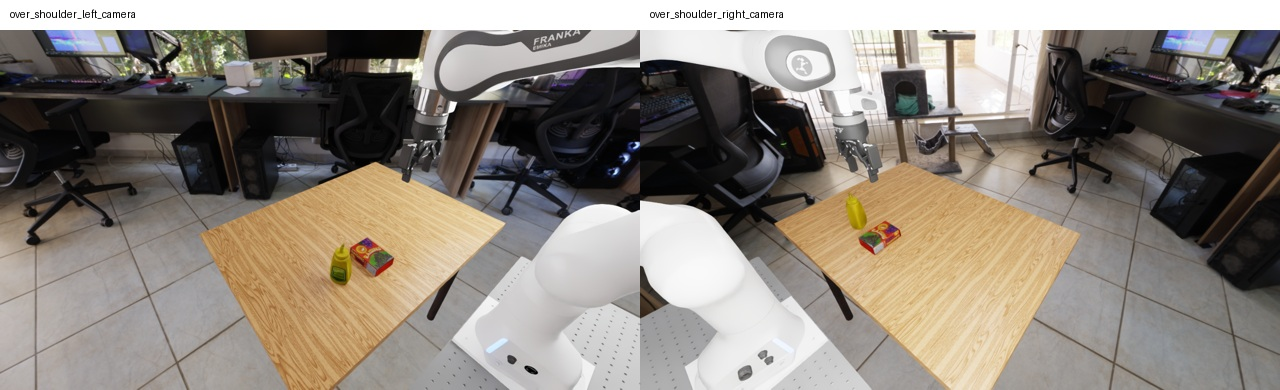
\includegraphics[width=\linewidth]{rev_scene_mustard.jpg}
\end{minipage}\hfill
\begin{minipage}[c]{.69\linewidth}
\textbf{Goal:} mustard to the right of the box.\par
TF and RF differ in the subject of the spatial clause. Both still ask the robot to move the mustard.
\end{minipage}\par\medskip
\begin{tabular}{@{}p{.20\linewidth}p{.76\linewidth}@{}}
\toprule
\textbf{Form} & \textbf{Exact instruction} \\
\midrule
Direct (DIR) & Place the mustard bottle on the table to the right of the raisin box. \\
\addlinespace
\textcolor{mover}{Target-first (TF)} & Move the mustard bottle on the table so that \textbf{the mustard bottle} is to the right of the raisin box. \\
\addlinespace
\textcolor{reference}{Reference-first (RF)} & Move the mustard bottle on the table so that \textbf{the raisin box} is to the left of the mustard bottle. \\
\bottomrule
\end{tabular}
\end{table}

\section{Paired Spatial Evaluation}
To test whether wording changes behavior without changing the task, we repeat each placement from the same physical start under three instructions. We compare how often the requested arrangement is reached, then examine whether that score captures the intended manipulation and its final outcome.

\begin{samepage}
We use four tabletop scenes from RoboLab, a simulation benchmark for generalist manipulation policies~\citep{yang2026robolab}. The cube scene asks the robot to place a cube left, right, in front of, or behind a bowl. The butter and mustard scenes each ask it to place that object left, right, or on top of a raisin box. The bowl scene asks it to stack either bowl on the other. Seven goals are provided by RoboLab, and five extend the same scenes without changing their objects (Appendix~\ref{app:tasks}).
\par
\end{samepage}

Table~\ref{tab:setup} illustrates the three instruction forms using the same mustard-placement goal. The direct form (DIR) is a concise command that retains RoboLab's original wording where available. Target-first (TF) expands the command by describing the mustard as right of the box. Reference-first (RF) instead describes the box as left of the mustard, while still asking the robot to move the mustard. Comparing TF with RF tests this change in perspective; comparing DIR with TF tests the expansion itself. The DIR--RF comparison combines both changes and appears in Appendix~\ref{app:behavior-results}. For bowl stacking, ``underneath and supporting'' is less specific than the nesting required by the scorer, so we also analyze the results without these goals.

We evaluate the DROID versions of Cosmos3 Nano, Cosmos3 Edge, and FLUX 3 Action~\citep{nvidia2026nano,nvidia2026edge,bfl2026fluxaction}. Nano and FLUX were selected for strong RoboLab performance, with Edge providing a smaller Cosmos comparison~\citep{robolab2026leaderboard}. Each receives wrist and two exterior camera views plus the robot's proprioceptive state. We vary object poses to obtain eight starts per scene that a scripted controller can solve. For every model and goal, we reset the robot and objects before each instruction, so all three wordings receive identical initial observations. These are our \emph{paired runs}. The resulting 864 episodes last 20--40 seconds, including continued control after placement (Appendix~\ref{app:settings}).

We measure the proportion of runs that reach a \emph{stable placement}: the requested relation must hold for one second while the target is supported, moves slower than 2\,cm/s, and does not touch the gripper. Directions use the robot's coordinate frame. Checking these conditions at any time and again during the final second distinguishes reaching an arrangement from retaining it. Neither check identifies which object moved, however. A cube can end up behind a bowl because the robot moves the cube backward or the bowl forward.

For each model and goal, we compare the outcomes under different wordings from the same starts. We average over goals within scenes, then give each scene and model equal weight. A positive TF--RF difference therefore means that more runs reach the placement under TF. Uncertainty reflects the shared starts rather than treating all rollouts as independent. Three goals already hold initially; they are hatched in Fig.~\ref{fig:goals}, and we also report rates excluding them (Appendices~\ref{app:statistics} and~\ref{app:counts}).

\section{Results}
Task competence under one description does not guarantee consistency across equivalent instructions. Across the three models, the proportion of runs reaching a stable placement is 12.2 percentage points higher under TF than RF (95\% interval 8.6--15.4, adjusted $p<0.001$; Fig.~\ref{fig:wording}). This advantage appears in all three models even though each wording requests the same manipulation from the same physical start. TF and RF do change both object order and relation vocabulary, so this comparison does not identify which aspect drives the effect.

\begin{figure}[!ht]
\centering
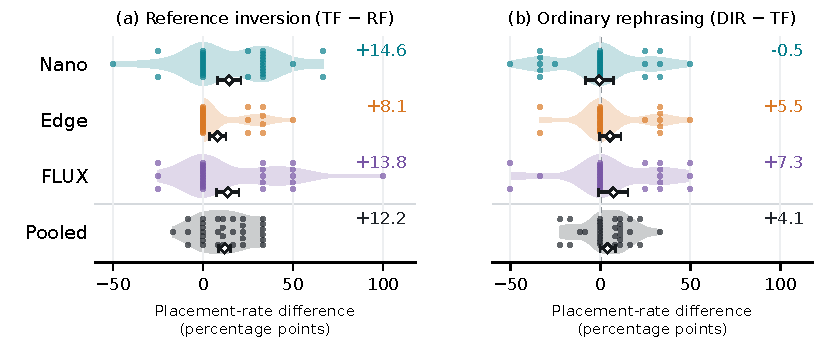
\includegraphics[width=\linewidth]{rev_wording_effect.pdf}
\caption{Wording effects across 32 physical starts. Dots show start-level average differences; diamonds and bars show means and 95\% intervals. Positive TF--RF favors target-first wording. Wider sections indicate more starts with similar effects.}
\label{fig:wording}
\end{figure}
\FloatBarrier

The average advantage does not provide a reliable prompting rule for every task. Placing mustard to the right of the box succeeds in 20 of 24 TF runs but only two RF runs. In the cube scene, however, effects in opposite directions cancel: RF performs better for cube-behind despite the scene's zero average gap (Fig.~\ref{fig:goals}). An aggregate score can therefore hide sensitivity to individual relations. The overall TF advantage also persists when the ambiguous bowl-stacking goals are removed (Appendix~\ref{app:statistics}).

\begin{figure}[!htb]
\centering
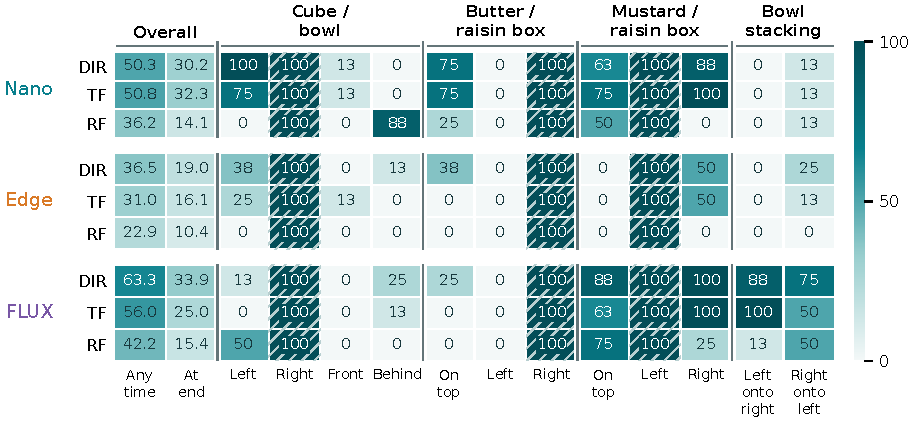
\includegraphics[width=\linewidth]{rev_goal_response_by_form.pdf}
\caption{Stable-placement rates (\%). Overall columns weight goals equally within scenes and scenes equally. Each row contains 96 episodes; each goal uses eight starts. Hatched goals already hold initially and remain included. The scores check the arrangement, not which object moved.}
\label{fig:goals}
\end{figure}



A scored arrangement does not necessarily mean the robot followed the instruction. In one Nano rollout, the cube ends up behind the bowl because the robot moves the bowl rather than the requested cube (Appendix~\ref{app:executions}). Arrangements can also be lost: the overall placement rate falls from 43.2\% at any time to 21.8\% at episode end. Evaluation must therefore verify which object moved and whether the requested arrangement was retained.

\FloatBarrier
\section{Interpreting the Requested Goal}
To separate instruction interpretation from action generation, we tested each policy's language model on the same ten cube, butter, and mustard goals (Fig.~\ref{fig:vqa-protocol}). We compare text alone with initial images from eight starts per scene; Appendix~\ref{app:vqa} details the protocol and controls.

\begin{figure}[!ht]
\centering
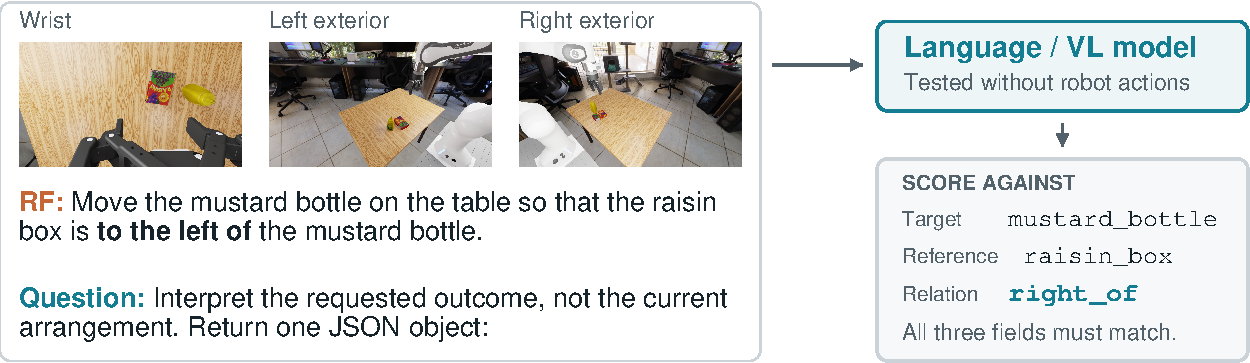
\includegraphics[width=\linewidth]{rev_vqa_protocol.pdf}
\caption{Instruction-understanding test with an exact RF example and question excerpt. Answers must describe the requested outcome. Text-only queries omit images; camera descriptions and vocabulary lists are omitted here.}
\label{fig:vqa-protocol}
\end{figure}

\begin{table}[!ht]
\centering\small
\caption{Instruction accuracy under constrained decoding: correct out of ten (text) or equal-scene percentage (images + camera descriptions). $\dagger$ FLUX's image scores test standalone Qwen; the policy uses Qwen for text only.}
\label{tab:vqa}
\begin{tabular}{@{}llcc@{\quad}cc@{}}
\toprule
& & \multicolumn{2}{c}{Text only (/10)} & \multicolumn{2}{c}{With images (\%)}\\
Policy & Language model tested & TF & RF & TF & RF\\
\midrule
Nano & Qwen3-VL-8B-Instruct & 10 & 10 & 100.0 & 89.9\\
Edge & Cosmos3-Edge reasoner & 8 & 4 & 48.3 & 23.3\\
FLUX & Qwen3-VL-4B-Instruct & 10 & 4 & $100.0^\dagger$ & $41.7^\dagger$\\
\bottomrule
\end{tabular}
\end{table}

Reference-first instructions can be misinterpreted even when the language model is evaluated on its own. For example, FLUX correctly identifies the mustard and box but interprets the RF instruction in Table~\ref{tab:setup} as requiring the mustard to be \emph{left} of the box. It reverses the relation in all six text-only RF errors. Edge also interprets fewer RF than TF instructions correctly (Table~\ref{tab:vqa}).

Understanding the text alone does not guarantee the same interpretation with images. Nano answers every text-only instruction correctly, but adding images and camera descriptions introduces errors on two RF instructions: RF accuracy falls to 89.9\% while TF remains correct. Camera descriptions alone change no answers. The tested language components do not consistently recover the same goal from equivalent spatial descriptions. This inconsistency may contribute to the wording-dependent failures observed in policy rollouts.

\section{Discussion and Conclusion}
Our results make instruction consistency a necessary complement to task performance. Following SIMPLER's controlled-simulation approach~\citep{li2025simpler}, repeating a task from the same physical start reveals failures that favorable wording can conceal. Opposing effects across relations also caution against treating TF as a universal prompting solution. Language interpretation errors do not establish the cause of a robot failure. The tested language-model weights match upstream or base checkpoints, so these errors cannot be attributed to changes in those weights during robot adaptation. Unavailable matched training data prevent a controlled comparison of training recipes or co-training.

% Visual arrangement judgments remain inconclusive, and their labels still require human review (Appendix~\ref{app:vqa}).

A correct spatial relation captures only part of instruction following, just as LIBERO-CF distinguishes object contact from task success~\citep{fang2026counterfactual}. Broader scenes are needed to establish how common these failures are. Evaluation can nevertheless address them by testing several descriptions per goal, checking which object moved, and verifying the final arrangement.

\clearpage
\bibliography{references}
\clearpage
\appendix

\setlength{\parskip}{5.5pt}
% Insert after references, with \appendix already issued by the parent document.
% Requires graphicx, booktabs, longtable, array. Figure paths can be adjusted when copied.
\section{Evaluation details and full instructions}
\label{app:tasks}
The comparison changes the instruction while fixing the requested placement and the object the robot should move. For each physical starting state, the same model is run separately under the direct (DIR), target-first (TF), and reference-first (RF) instructions. ``Target-first'' describes the order of objects in the relational clause after ``so that''. Every instruction still names the same target object as the object to move. The control sequence is not fixed: each policy generates a new sequence from its instruction, so later observations may differ.

\subsection{Scenes and starting states}
The study includes eight starting states in each of four native RoboLab scenes. Small changes to object positions and orientations produce different starts, and a scripted controller checks the requested placements before learned-policy evaluation. The cube scene has four goals, each box scene has three, and the two-bowl scene has two, giving twelve goals and 36 instructions. With three models and eight starts for every goal, this yields 864 episodes. The planned two-bin scene did not produce a qualifying start with the scripted controller and was excluded before the learned-policy outcomes were collected. It contributes no observations to these results.

\begin{table}[htbp]
\centering\small
\caption{Scenes, goals, and episode duration. All goals in a scene share its eight starting states. The already-satisfied column describes all eight starts in that scene.}
\label{tab:appendix-scenes}
\begin{tabular}{@{}p{.25\linewidth}p{.36\linewidth}p{.20\linewidth}r@{}}
\toprule Scene & Requested placements & Already satisfied & Duration\\
\midrule
Cube and bowl & Cube left, right, in front, behind bowl & Cube right & 30\,s\\
Butter and raisin box & Butter left, right, on top of box & Butter right & 40\,s\\
Mustard and raisin box & Mustard left, right, on top of box & Mustard left & 40\,s\\
Two bowls & Either bowl on the other & None & 20\,s\\
\bottomrule
\end{tabular}
\end{table}

Directions are defined in the robot's coordinate frame. The left and right bowl identities are assigned from their positions at reset and remain fixed for the episode. Seven goals are supplied by RoboLab, and five add left/right placements using these same scenes and objects. In particular, the cube-right instruction is tested in the simple cube/bowl/banana scene used for the other cube goals, rather than in RoboLab's separate cube-right scene with additional objects.

\begin{figure}[htbp]
\centering
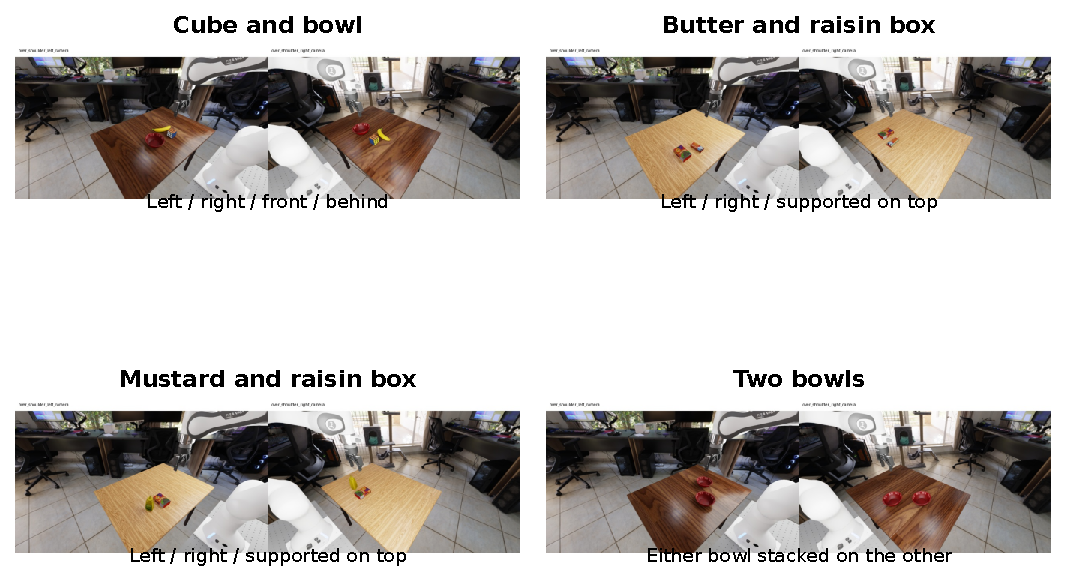
\includegraphics[width=\linewidth]{rev_scene_overview.pdf}
\caption{The four scene assets used in the study. These pilot views illustrate the objects and workspace. They are not the exact confirmation resets. All wording comparisons within a start use identical physical states.}
\label{fig:scene-overview}
\end{figure}
\FloatBarrier
\subsection{Exact instructions}
Tables below reproduce all tested instructions. DIR retains the benchmark task's original wording where that goal exists on the scene. It is a baseline instruction, not evidence that wording came from a diverse human annotation process. TF describes the relation starting with the target object, whereas RF starts with the reference object and reverses the relation. The source file preserves a trailing space in the native mustard-on-box instruction. That whitespace is omitted from this typeset table.

\subsubsection{Cube and bowl}

\begin{longtable}{@{}p{.08\linewidth}p{.87\linewidth}@{}}
\toprule Form & Instruction\\\midrule\endhead

\multicolumn{2}{@{}l}{\textbf{Cube left of bowl}}\\

DIR & Put the rubiks cube to the left of the bowl\\[3pt]

TF & Place the Rubik's cube so that the Rubik's cube is to the left of the bowl.\\[3pt]

RF & Place the Rubik's cube so that the bowl is to the right of the Rubik's cube.\\[3pt]

\addlinespace

\multicolumn{2}{@{}l}{\textbf{Cube right of bowl}}\\

DIR & Put the rubiks cube to the right of the bowl\\[3pt]

TF & Place the Rubik's cube so that the Rubik's cube is to the right of the bowl.\\[3pt]

RF & Place the Rubik's cube so that the bowl is to the left of the Rubik's cube.\\[3pt]

\addlinespace

\multicolumn{2}{@{}l}{\textbf{Cube in front of bowl}}\\

DIR & Put the rubiks cube in front of the bowl\\[3pt]

TF & Place the Rubik's cube so that the Rubik's cube is in front of the bowl.\\[3pt]

RF & Place the Rubik's cube so that the bowl is behind the Rubik's cube.\\[3pt]

\addlinespace

\multicolumn{2}{@{}l}{\textbf{Cube behind bowl}}\\

DIR & Put the rubiks cube behind the bowl\\[3pt]

TF & Place the Rubik's cube so that the Rubik's cube is behind the bowl.\\[3pt]

RF & Place the Rubik's cube so that the bowl is in front of the Rubik's cube.\\[3pt]

\addlinespace

\bottomrule\end{longtable}

\subsubsection{Butter and raisin box}

\begin{longtable}{@{}p{.08\linewidth}p{.87\linewidth}@{}}
\toprule Form & Instruction\\\midrule\endhead

\multicolumn{2}{@{}l}{\textbf{Butter box on raisin box}}\\

DIR & Pick up the butter box and place it on top of the raisin box\\[3pt]

TF & Place the butter box so that the butter box is on top of and supported by the raisin box.\\[3pt]

RF & Place the butter box so that the raisin box is underneath and supporting the butter box.\\[3pt]

\addlinespace

\multicolumn{2}{@{}l}{\textbf{Butter box left of raisin box}}\\

DIR & Place the butter box on the table to the left of the raisin box.\\[3pt]

TF & Move the butter box on the table so that the butter box is to the left of the raisin box.\\[3pt]

RF & Move the butter box on the table so that the raisin box is to the right of the butter box.\\[3pt]

\addlinespace

\multicolumn{2}{@{}l}{\textbf{Butter box right of raisin box}}\\

DIR & Place the butter box on the table to the right of the raisin box.\\[3pt]

TF & Move the butter box on the table so that the butter box is to the right of the raisin box.\\[3pt]

RF & Move the butter box on the table so that the raisin box is to the left of the butter box.\\[3pt]

\addlinespace

\bottomrule\end{longtable}

\subsubsection{Mustard and raisin box}

\begin{longtable}{@{}p{.08\linewidth}p{.87\linewidth}@{}}
\toprule Form & Instruction\\\midrule\endhead

\multicolumn{2}{@{}l}{\textbf{Mustard bottle on raisin box}}\\

DIR & Place the mustard on the raisin box.\\[3pt]

TF & Place the mustard bottle so that the mustard bottle is on top of and supported by the raisin box.\\[3pt]

RF & Place the mustard bottle so that the raisin box is underneath and supporting the mustard bottle.\\[3pt]

\addlinespace

\multicolumn{2}{@{}l}{\textbf{Mustard bottle left of raisin box}}\\

DIR & Place the mustard bottle on the table to the left of the raisin box.\\[3pt]

TF & Move the mustard bottle on the table so that the mustard bottle is to the left of the raisin box.\\[3pt]

RF & Move the mustard bottle on the table so that the raisin box is to the right of the mustard bottle.\\[3pt]

\addlinespace

\multicolumn{2}{@{}l}{\textbf{Mustard bottle right of raisin box}}\\

DIR & Place the mustard bottle on the table to the right of the raisin box.\\[3pt]

TF & Move the mustard bottle on the table so that the mustard bottle is to the right of the raisin box.\\[3pt]

RF & Move the mustard bottle on the table so that the raisin box is to the left of the mustard bottle.\\[3pt]

\addlinespace

\bottomrule\end{longtable}

\clearpage
\subsubsection{Two bowls}

\begin{longtable}{@{}p{.08\linewidth}p{.87\linewidth}@{}}
\toprule Form & Instruction\\\midrule\endhead

\multicolumn{2}{@{}l}{\textbf{Left bowl onto right bowl}}\\

DIR & Stack the left bowl on the right bowl\\[3pt]

TF & Move the left bowl so that the left bowl is stacked on the right bowl.\\[3pt]

RF & Move the left bowl so that the right bowl is underneath and supporting the left bowl.\\[3pt]

\addlinespace

\multicolumn{2}{@{}l}{\textbf{Right bowl onto left bowl}}\\

DIR & Stack the right bowl on the left bowl\\[3pt]

TF & Move the right bowl so that the right bowl is stacked on the left bowl.\\[3pt]

RF & Move the right bowl so that the left bowl is underneath and supporting the right bowl.\\[3pt]

\addlinespace

\bottomrule\end{longtable}


The bowl task deserves separate interpretation. Its DIR instruction requests stacking, and its TF instruction likewise specifies that the target is stacked on the other bowl. RF describes the lower bowl as underneath and supporting the target bowl. That wording does not explicitly require the nesting checked by the benchmark predicate. The bowl results are therefore reported separately and the pooled wording contrast is also examined without them.

\section{Policy settings and evaluation criteria}\label{app:settings}
The policies receive one camera view attached to the wrist, two fixed exterior views overlooking the workspace, and robot state. We retain RoboLab's native camera configuration across all wording conditions. No camera is repositioned for a particular instruction. Each request returns 32 actions, executed at 15\,Hz before the next observation and request. The final chunk is truncated at the episode horizon. The same request seed (6100) is used for the paired instructions. Episodes run for the complete duration in Table~\ref{tab:appendix-scenes}, even after a placement first passes the check. There are no automatic request retries. The policy implementation and camera preprocessing remain specific to each released checkpoint.

\begin{table}[htbp]
\centering\small
\caption{Recorded inference settings. Values come from the policy server receipts used in the study.}
\label{tab:appendix-settings}
\begin{tabular}{@{}lccc@{}}
\toprule Setting & Cosmos3 Nano & Cosmos3 Edge & FLUX 3 Action\\
\midrule
Arithmetic & bfloat16 & bfloat16 & bfloat16\\
Sampling steps & 4 & 4 & 4\\
Sampler & UniPC & UniPC & Cosmos UniPC\\
Noise shift & 5.0 & 5.0 & 5.0\\
Visual guidance & 3.0 & 3.0 & 4.0\\
Action guidance & --- & --- & 1.0\\
Observation history & 1 & 1 & 1\\
Actions per request & 32 & 32 & 32\\
Control frequency & 15\,Hz & 15\,Hz & 15\,Hz\\
Prompt JSON formatting & No & Yes & No\\
Input/canvas setting & $540\!\times\!640$ & $540\!\times\!640$ & $544\!\times\!736$\\
\bottomrule
\end{tabular}
\end{table}

The Cosmos models use joint-position actions and a \texttt{480} resolution setting. Edge records a guidance interval of [960,1001]. FLUX uses its DROID camera layout and absolute action parameterization with the released action scale of 2.0. FLUX's immutable configuration retains an inference-seed value of 0, while each inference call explicitly supplies the study seed 6100. This overrides the configuration value. Canvas dimensions are model-specific preprocessing settings, not different simulated camera placements. Full recorded configurations and release identities are preserved in the accompanying reproducibility files. The original compact FLUX receipt lacks a revision identifier, so a complete executed-policy manifest remains unavailable. The later component audit verifies the narrower shared-encoder identity (Appendix~\ref{app:vqa}).

\subsection{Placement criteria and statistical comparison}\label{app:statistics}
For left/right/front/behind, the spatial predicate uses the native 45-degree relation cone in the robot frame and requires the target to be supported by the table. For on-top placement, the native support predicate checks upward support and the target centroid within the reference footprint, with a 1\,cm tolerance. Bowl stacking combines the native open-top containment predicate with contact between the bowls. In every case the gripper must be detached from the target. A stable placement requires the full predicate and target speed below 2\,cm/s for one continuous second. Speed is computed by a backward difference of successive recorded positions at 15\,Hz, which avoids treating solver velocity jitter at an unchanged position as motion.

The any-time outcome asks whether this condition holds anywhere in the episode. The episode-end outcome requires it throughout the final second. Neither condition proves that the intended object was manipulated. For example, moving the reference can make the requested relative arrangement true while leaving the target untouched. They are placement outcomes rather than a complete instruction-following score.

The saved initial states determine whether a requested arrangement holds before any policy action. Cube-right, butter-right, and mustard-left are initially satisfied in all eight starts. Those three goals account for 216 episodes, and the other nine account for 648 episodes. Every initially-satisfied episode passes the any-time criterion, so including these episodes increases absolute any-time rates without changing their TF--RF contribution, which is zero. Earlier per-episode labels disagreed with the saved-state classification for 44 episodes. The supplementary table uses the common saved-state labels consistently across forms and models. Original any-time and episode-end outcomes are unchanged.

For a wording comparison, the two binary placement outcomes are subtracted for the same model, starting state, and goal. For example, if TF reaches the placement and RF does not, the paired difference is +1. The reverse gives $-1$, and agreement gives 0. Differences are averaged over goals within each scene, then equally over scenes and models. This prevents scenes with more goals from dominating the pooled result. Confidence intervals use 10,000 bootstrap draws of the eight physical starts within each scene. All associated goals, models, and instruction forms remain together. The original pooled TF--RF and DIR--TF tests use paired sign flips and Holm correction across those two tests. Per-model, subgroup, per-relation, terminal-outcome, and newly added DIR--RF summaries are descriptive. They do not expand that original test family.

The pooled TF--RF estimate is 12.15 percentage points for any-time placement and 11.20 points for episode-end placement. Removing the bowl scene and giving each remaining scene equal weight leaves an any-time estimate of 10.65 points. This descriptive sensitivity check shows that the main direction does not depend on the bowl-language ambiguity. It does not establish equivalence of the bowl prompts. DIR--TF is 4.08 points, with a 95\% interval of $[-0.2,8.4]$ and an adjusted $p=0.089$. Failure to detect that difference is not evidence that instruction expansion has no effect.

\section{Additional behavioral results}
\label{app:behavior-results}
\subsection{Direct versus reference-first wording}
The direct baseline can also be compared with reference-first wording. This added comparison is useful for connecting the controlled TF--RF intervention to the short instruction normally supplied with a task, but DIR and RF also differ in length and sentence construction. It therefore does not isolate reference reversal as closely as TF versus RF. Table~\ref{tab:appendix-di} and Figure~\ref{fig:appendix-di} report it descriptively.
\begin{table}[htbp]
\centering\small
\caption{Exploratory DIR--RF gaps in percentage points, with 95\% intervals obtained by resampling paired physical starts. Positive values favor the direct instruction. No new multiplicity-adjusted significance claims are made.}
\label{tab:appendix-di}
\begin{tabular}{@{}lcc@{}}\toprule Model & At any time & At episode end\\\midrule

All models & 16.2 [11.7, 20.4] & 14.4 [10.0, 18.9]\\

Nano & 14.1 [7.0, 20.8] & 16.1 [4.2, 27.6]\\

Edge & 13.5 [7.8, 19.5] & 8.6 [0.0, 17.7]\\

FLUX & 21.1 [10.4, 30.7] & 18.5 [9.1, 27.6]\\

\bottomrule\end{tabular}\end{table}

\begin{figure}[htbp]\centering
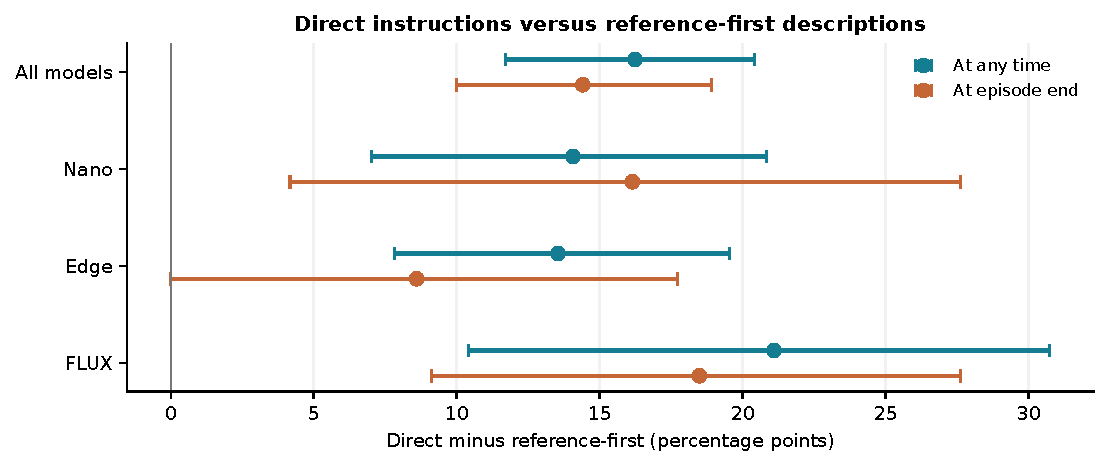
\includegraphics[width=.90\linewidth]{rev_direct_reference_effects.pdf}
\caption{The short direct instruction also outperforms reference-first descriptions on average. Intervals are descriptive paired-start bootstrap intervals. DIR--RF was added after the original analyses.}
\label{fig:appendix-di}\end{figure}

\subsection{Relation-specific effects}
Figure~\ref{fig:appendix-relation} shows that the average wording effect does not represent a uniform drop across relations. Mustard-right exhibits the largest contrast: 20 of 24 target-first episodes reach the placement, compared with 2 of 24 reference-first episodes. These counts pool the three models over eight starts each. The corresponding target-first/reference-first counts are 8/0 for Nano, 4/0 for Edge, and 8/2 for FLUX. By contrast, cube-behind has a negative TF--RF gap, and the cube scene has no net TF--RF gap after averaging its four relations. This pattern motivates testing equivalent descriptions within each relation rather than expecting one prompt form to be uniformly preferable. Per-relation estimates involve only eight physical starts and should be read as descriptive localization of the observed effect.

\begin{figure}[htbp]\centering
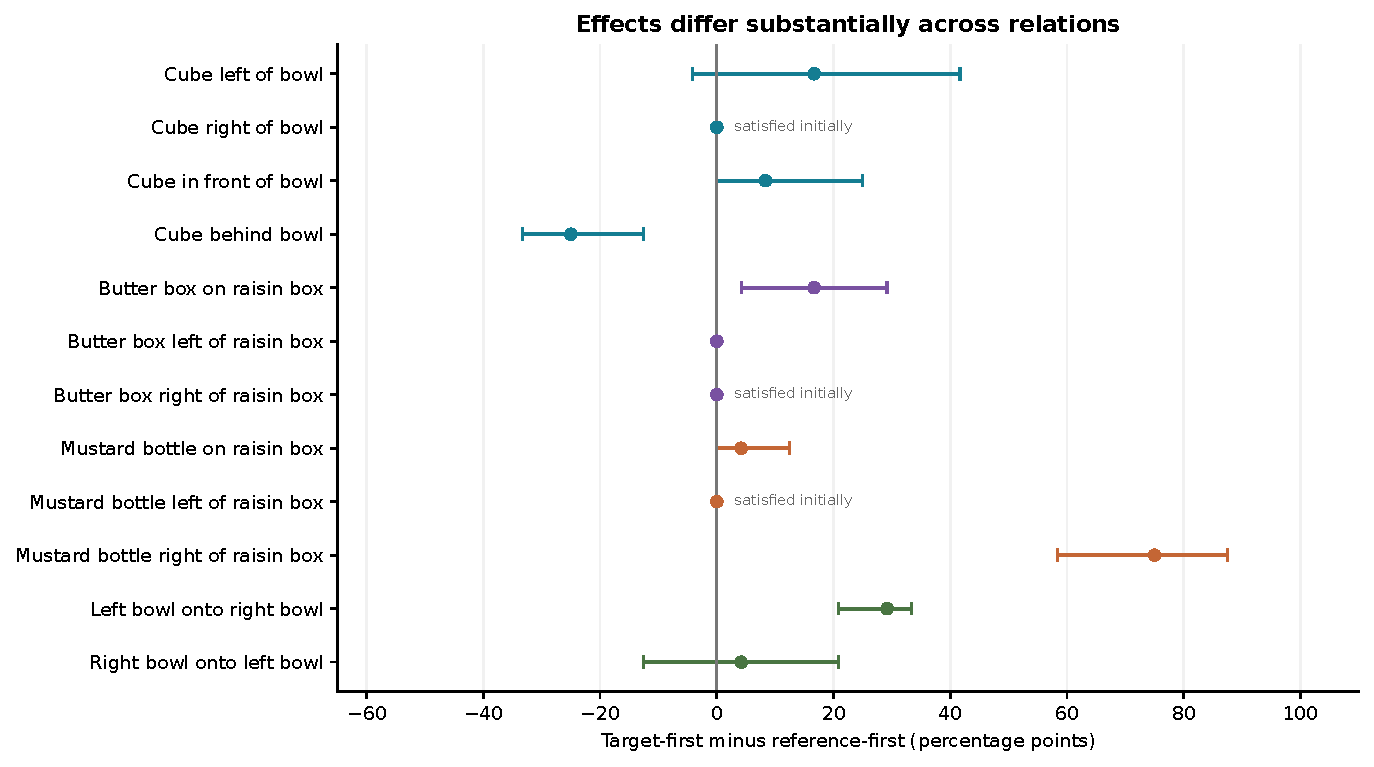
\includegraphics[width=\linewidth]{rev_per_relation_effects.pdf}
\caption{Per-relation TF--RF differences pooled over models, with descriptive 95\% intervals from the eight physical starts for that scene. Positive values favor target-first wording. Initially-satisfied goals contribute zero to this any-time contrast.}
\label{fig:appendix-relation}\end{figure}

\subsection{Reaching an arrangement and keeping it}
Across the 864 episodes, 383 reach a stable placement and 191 also satisfy the episode-end criterion. Thus 192 of the 383 any-time passes (50.1\%) do not retain the scored arrangement through the final second. Among the 648 episodes that must establish a new arrangement, 167 reach it and 94 retain it at the end. The remaining 73 account for 43.7\% of that group's any-time passes. For initially-satisfied goals, 97 of 216 episodes preserve a final stable outcome. These are raw counts. Figure~\ref{fig:appendix-end} uses the scene-balanced rates used in the main paper, so its percentages need not equal the raw fractions.

\begin{figure}[htbp]\centering
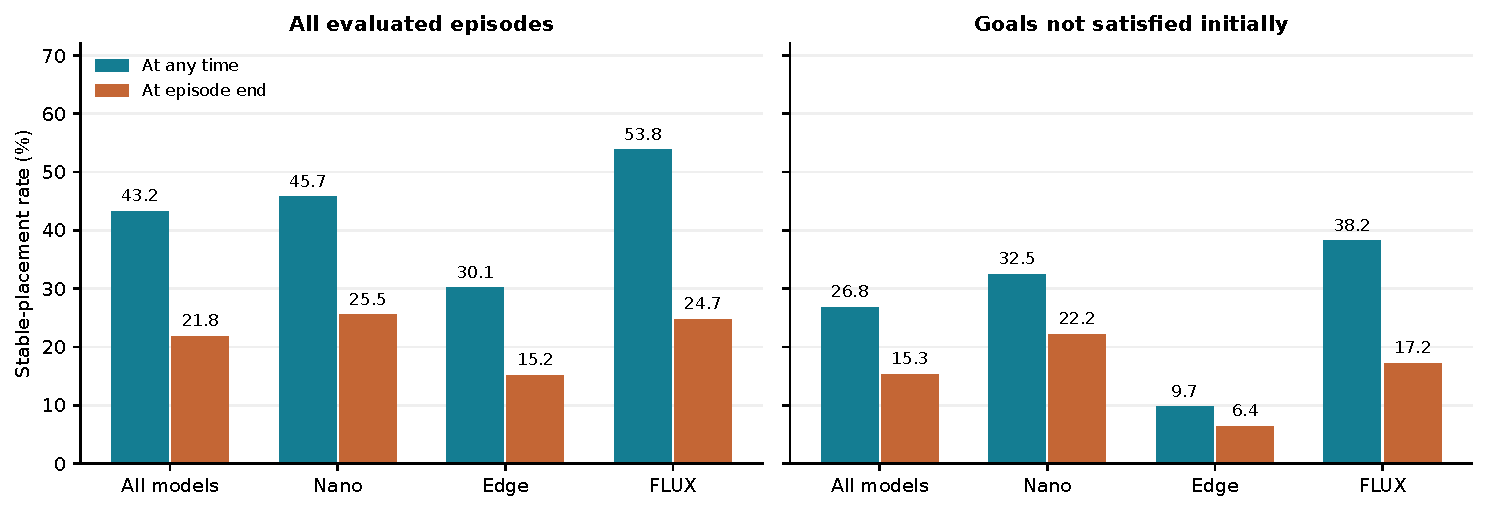
\includegraphics[width=\linewidth]{rev_anytime_end.pdf}
\caption{Any-time and episode-end placement rates, averaging goals within each scene and weighting scenes equally. The right panel excludes goals already satisfied at reset. Reaching the scored arrangement and keeping it under continued control are distinct requirements.}
\label{fig:appendix-end}\end{figure}

\subsection{Complete per-goal counts}\label{app:counts}
Each table entry gives the number of any-time passes followed by the number of episode-end passes, both out of eight starts. A dagger marks a goal satisfied at all eight initial states. No missing observations are represented as zero. These tables report the original physical outcome predicates, not a newly corrected measure of instruction success.

\begin{table}[htbp]\centering\small
\caption{Nano placement counts. Entries are any-time/end, each out of eight.}
\begin{tabular}{@{}p{.48\linewidth}ccc@{}}\toprule Goal & Direct & Target-first & Reference-first\\\midrule

Cube left of bowl & 8/2 & 6/3 & 0/0\\

Cube right of bowl$^\dagger$ & 8/3 & 8/2 & 8/0\\

Cube in front of bowl & 1/1 & 1/1 & 0/0\\

Cube behind bowl & 0/0 & 0/0 & 7/6\\

Butter box on raisin box & 6/5 & 6/5 & 2/1\\

Butter box left of raisin box & 0/0 & 0/0 & 0/0\\

Butter box right of raisin box$^\dagger$ & 8/5 & 8/4 & 8/6\\

Mustard bottle on raisin box & 5/5 & 6/5 & 4/2\\

Mustard bottle left of raisin box$^\dagger$ & 8/5 & 8/5 & 8/0\\

Mustard bottle right of raisin box & 7/3 & 8/6 & 0/0\\

Left bowl onto right bowl & 0/0 & 0/0 & 0/0\\

Right bowl onto left bowl & 1/1 & 1/1 & 1/0\\

\bottomrule\end{tabular}\end{table}

\begin{table}[htbp]\centering\small
\caption{Edge placement counts. Entries are any-time/end, each out of eight.}
\begin{tabular}{@{}p{.48\linewidth}ccc@{}}\toprule Goal & Direct & Target-first & Reference-first\\\midrule

Cube left of bowl & 3/1 & 2/1 & 0/0\\

Cube right of bowl$^\dagger$ & 8/4 & 8/3 & 8/0\\

Cube in front of bowl & 0/0 & 1/0 & 0/0\\

Cube behind bowl & 1/0 & 0/0 & 0/0\\

Butter box on raisin box & 3/2 & 0/0 & 0/0\\

Butter box left of raisin box & 0/0 & 0/0 & 0/0\\

Butter box right of raisin box$^\dagger$ & 8/5 & 8/3 & 8/7\\

Mustard bottle on raisin box & 0/0 & 0/0 & 0/0\\

Mustard bottle left of raisin box$^\dagger$ & 8/3 & 8/4 & 8/3\\

Mustard bottle right of raisin box & 4/3 & 4/4 & 0/0\\

Left bowl onto right bowl & 0/0 & 0/0 & 0/0\\

Right bowl onto left bowl & 2/1 & 1/1 & 0/0\\

\bottomrule\end{tabular}\end{table}

\begin{table}[htbp]\centering\small
\caption{FLUX placement counts. Entries are any-time/end, each out of eight.}
\begin{tabular}{@{}p{.48\linewidth}ccc@{}}\toprule Goal & Direct & Target-first & Reference-first\\\midrule

Cube left of bowl & 1/0 & 0/0 & 4/3\\

Cube right of bowl$^\dagger$ & 8/2 & 8/2 & 8/8\\

Cube in front of bowl & 0/0 & 0/0 & 0/0\\

Cube behind bowl & 2/0 & 1/0 & 0/0\\

Butter box on raisin box & 2/2 & 0/0 & 0/0\\

Butter box left of raisin box & 0/0 & 0/0 & 0/0\\

Butter box right of raisin box$^\dagger$ & 8/4 & 8/6 & 8/3\\

Mustard bottle on raisin box & 7/2 & 5/2 & 6/2\\

Mustard bottle left of raisin box$^\dagger$ & 8/6 & 8/4 & 8/0\\

Mustard bottle right of raisin box & 8/8 & 8/3 & 2/0\\

Left bowl onto right bowl & 7/6 & 8/5 & 1/1\\

Right bowl onto left bowl & 6/0 & 4/0 & 4/0\\

\bottomrule\end{tabular}\end{table}

\FloatBarrier
\section{Policy rollout examples and image context}
\label{app:executions}
These policy rollouts illustrate the wording effect and a limitation of spatial scoring. The mustard-right pair shows different outcomes from the same initial state; the cube-behind pair shows a scored relation reached by moving the wrong object. Figure~\ref{fig:full-views} provides the full camera context for both pairs. These examples were selected from the recorded outcome differences before inspecting their videos. They illustrate possible behaviors and are not used to estimate their prevalence.

\subsection{An arrangement can be reached by moving the reference object}
Both Nano instructions ask the robot to move the cube behind the bowl. In the reference-first rollout, however, the robot holds the bowl while the cube remains on the tabletop. Moving the bowl changes the relative positions enough for the cube-behind check to pass. The target-first rollout does not pass that check. Thus, the reference-first score advantage in this example is not evidence of better instruction following: the predicate credits a relation that became true through manipulation of the wrong object.

\begin{figure}[!ht]
\centering
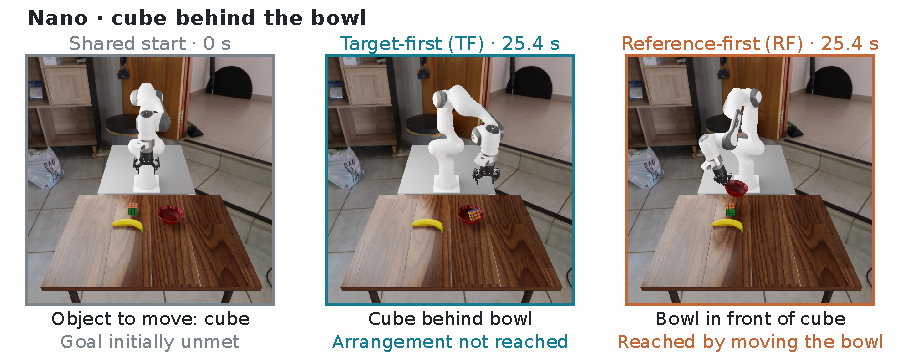
\includegraphics[width=\linewidth]{rev_execution_cube.pdf}
\caption{Nano's cube-behind policy rollouts. Both outcome snapshots are at 25.4 seconds, when the reference-first run first completes the stable-placement interval. The robot holds the bowl in RF while the cube is visible on the table. This arrangement no longer satisfies the episode-end check. The labels describe recorded spatial outcomes, not complete instruction success.}
\label{fig:wrong-object}
\end{figure}

\subsection{How the policy rollout panels were constructed}
The mustard pair uses Edge, the mustard-right goal, and physical start C02. The cube pair uses Nano, the cube-behind goal, and start C01. Each displayed pair shares the same initial physical state and uses a common snapshot time within that pair. Mustard snapshots are at 40 seconds, and cube snapshots are at 25.4 seconds. The original recordings were retrieved and checked against their saved file identities before frame extraction.

All main-paper and cropped appendix panels use the same image rectangle, taken from the exterior camera's original $1280\times720$ frame, followed by a 90-degree rotation for readability. The crop does not change within a pair or depend on the wording outcome. No objects or image content were generated or retouched. Figure~\ref{fig:full-views} shows the corresponding full frames in their native orientation. This preserves scene context and allows readers to see what the close views omit.

\begin{figure}[p]
\centering
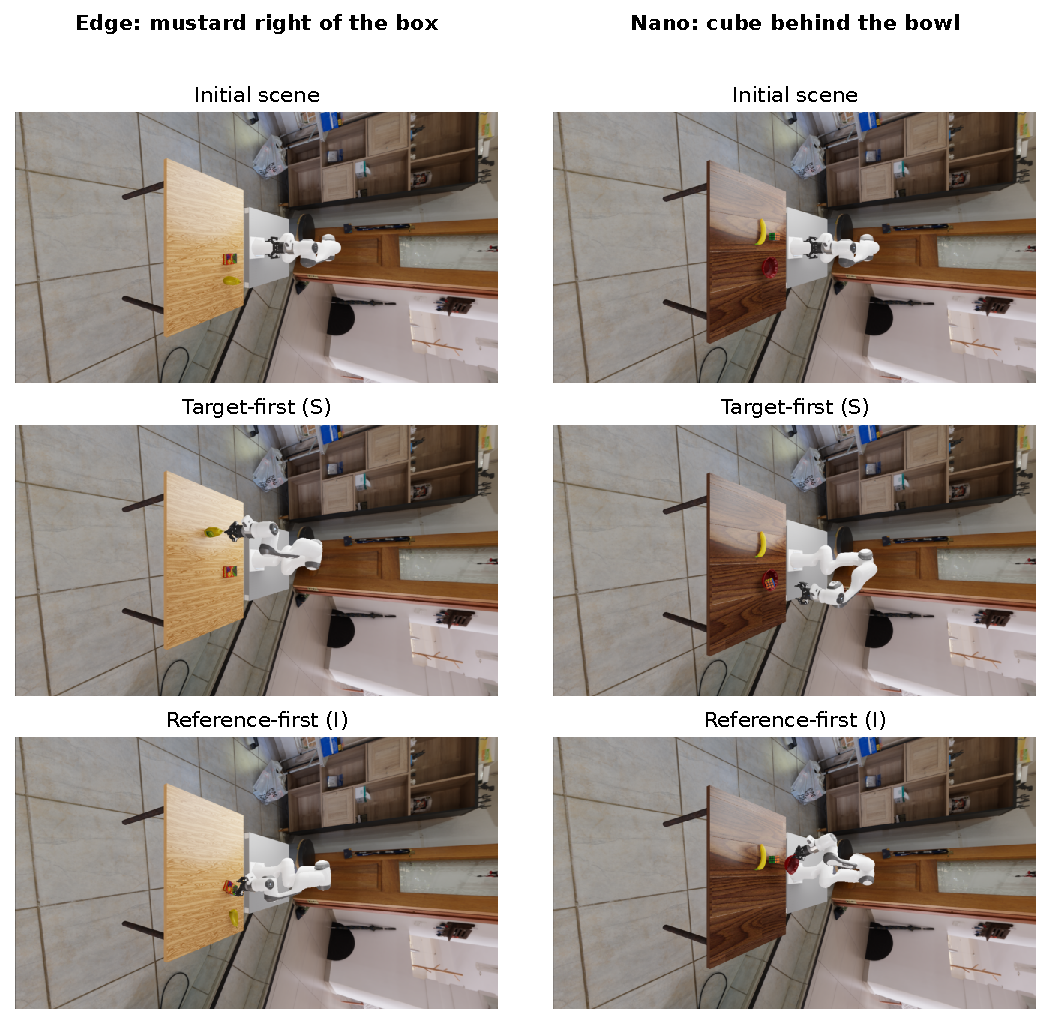
\includegraphics[width=\linewidth]{rev_full_execution_views.pdf}
\caption{Full exterior-camera frames for the two policy rollout examples. Columns correspond to Edge mustard-right and Nano cube-behind. Rows show the shared initial scene, TF, and RF. The camera image is shown in its native orientation, so image left/right should not be interpreted as the robot-frame relation. These are executed observations, not model-generated predictions.}
\label{fig:full-views}
\end{figure}

\clearpage
% Supplementary section for the separate Esmail revision. No edits to main.tex.
% Exact evidence map is in forecast_evidence_notes.md beside this file.
% Requires booktabs, graphicx. Tables fit the existing single-column CoRL style.
\section{Can predicted futures help explain a policy failure?}
\label{app:forecasts}

A generated future could make a world--action model easier to diagnose: it might show the wrong object moving before that error appears in the policy rollout. However, a forecast is useful for this purpose only if its content can be read reliably and it adds information beyond the current scene and proposed actions. We tested this additional diagnostic value on the recorded episodes. The automated annotation did not provide a measurable improvement. Low agreement between annotators, together with the absence of independent accuracy checks, leaves the information contained in the videos unresolved.

This was the study's original primary question. The wording comparisons in the main paper were planned secondary analyses and became the paper's focus after the behavioral outcomes were available. The original plan specified independent human annotation of generated videos. After viewing those outcomes, we replaced human annotation with two vision--language models (VLMs). This change was recorded before inspecting any VLM outputs. We report the forecast analysis here to preserve the full experimental record, including the limitations of that measurement procedure.

\begin{figure}[t]
\centering
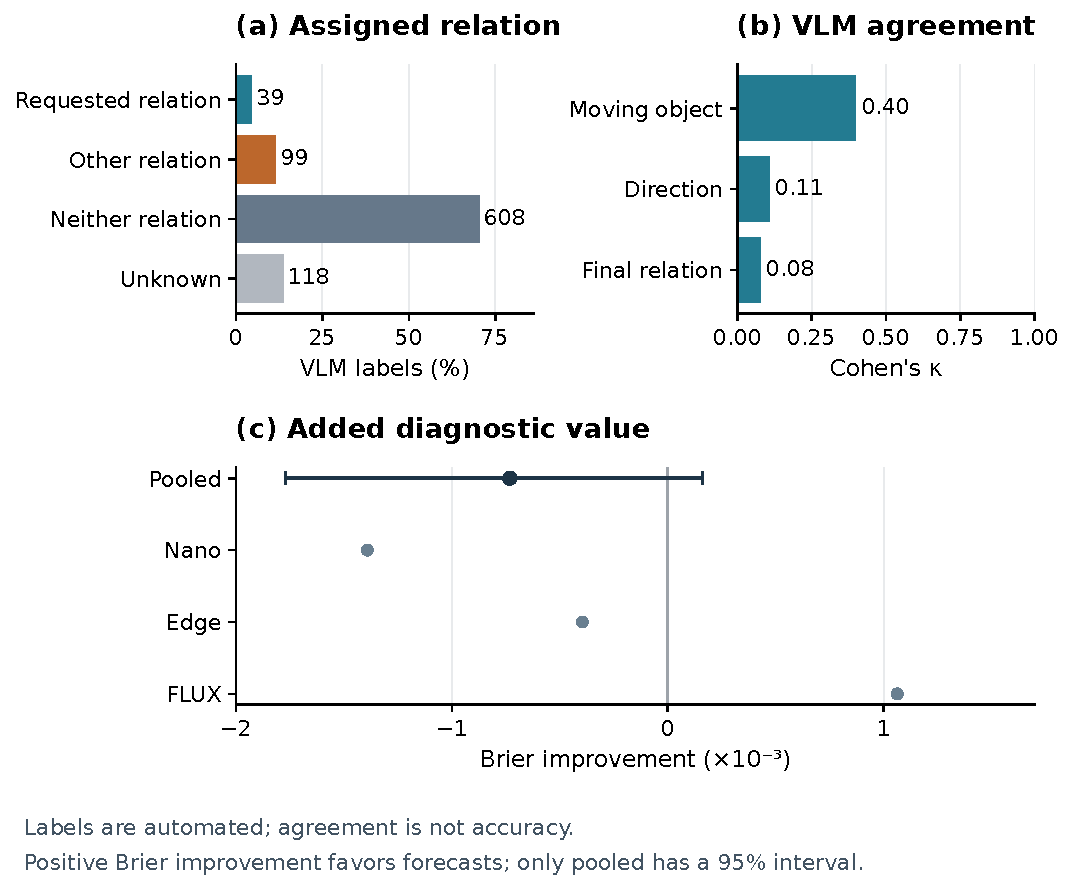
\includegraphics[width=\linewidth]{rev_forecast_diagnostics.pdf}
\caption{Three stages of the forecast diagnostic. (a) The relation assigned by the automated annotation. Numbers are counts of the 864 windows. Most labels identify neither the requested relation nor an alternative registered relation. (b) Independent VLM agreement on object identity, direction, and final relation. Agreement does not measure accuracy. (c) Change in held-out Brier error when forecast features are added. Positive values favor forecasts. Only the pooled estimate has a conditional 95\% interval. Complete export coverage does not establish reliable interpretation or added diagnostic value.}
\label{fig:forecast-measurement}
\end{figure}

\subsection{A forecast and its corresponding action segment}

The run records contain 13,968 saved futures across the 864 evaluation episodes. The diagnostic analysis uses one window per episode, selected without consulting the generated video or the later outcome. We select the first request for which the gripper is within 10\,cm of the surface of a movable task object. If no such request occurs, we use the episode's first request. This fallback was needed in two Nano episodes.

Each policy executes a chunk of up to 32 actions at 15\,Hz. The exported prediction comes from the same request as that action chunk. The annotation pipeline retains frames assigned to the executed part of the chunk, avoiding a comparison between an unexecuted suffix and behavior after a later replan. The implementation assigns forecast frame $k$ to $k/15$ seconds. For the two examples in Section~\ref{app:forecast-examples}, the model and export code establish this nominal correspondence, and the saved records verify the request, executed actions, and camera. These checks have not been extended to all 864 windows. Even a correct frame-to-action mapping does not establish that generated motion progresses at the executed pace, so this analysis is not a frame-by-frame forecast accuracy benchmark.

All 864 selected forecasts decoded. We also prepared the first-request clip when it differed from the selected window, yielding 1,726 annotation packets in total. A packet contains the episode's first observation with numbered objects and camera-orientation arrows, followed by the generated sequence. This legend can precede the selected request by one or more action chunks. The VLM sees eight evenly spaced frames, including the last retained frame. Frames are presented in a common layout: a wrist-camera view above two exterior views. The instruction, model name, requested goal, wording condition, policy rollout video, and task outcome are hidden. A common layout removes a simple model-identity cue, although visual rendering style may still reveal the generating model.

\subsection{What the automated annotators could read}

Two independent labelers, Qwen3-VL-235B-A22B-Instruct-FP8 and GLM-4.5V-FP8, identify the moving object, motion direction, visible final relation, reference object, possible release, and missing or hallucinated objects. The object labels are defined in the initial scene. Intended-goal compatibility is computed only after annotation. Unknown and ambiguous observations remain explicit labels. A video cannot establish contact forces or hidden three-dimensional containment from RGB alone.

When the labelers disagree, Qwen adjudicates between their two values and an unknown option, with the candidate order randomized. This procedure produces a complete derived table, but it does not turn agreement into ground truth: the adjudicator is also one of the original labelers. Both original label sets and raw responses are retained.

Agreement is weakest for the quantities needed to infer a destination (Table~\ref{tab:forecast-agreement}). Only 5.9\% of selected-window packets agree on every field. High raw agreement on possible release is also misleading because releases are rare. Its chance-corrected agreement is near zero. Neither averaging the annotators nor retaining only their agreements would by itself establish annotation accuracy.

\begin{table}[t]
\centering
\small
\begin{tabular}{lrr}
\toprule
Observable field & Agreement (\%) & Cohen's $\kappa$ \\
\midrule
Moving object & 59.1 & 0.398 \\
Motion direction & 48.6 & 0.108 \\
Visible final relation & 20.1 & 0.077 \\
Reference object for relation & 33.3 & 0.111 \\
Possible release & 93.4 & 0.026 \\
Missing object & 97.7 & 0.000 \\
Hallucinated object & 98.5 & 0.231 \\
\bottomrule
\end{tabular}
\caption{Independent VLM agreement on the 864 selected forecast windows. These are agreement measures, not accuracy estimates. The original labelers agree on all fields in 5.9\% of packets. Agreement is lower on the 862 additional first-request windows: $\kappa$ is at most 0.114 for every field.}
\label{tab:forecast-agreement}
\end{table}

The adjudicated labels describe upward-only motion in 673 of 864 windows (77.9\%). Only 39 windows (4.5\%) are assigned the requested final relation, 99 (11.5\%) another registered relation, 608 (70.4\%) neither, and 118 (13.7\%) an unknown relation. These are properties of the automated annotation, not independently established properties of the generated videos. They suggest a practical obstacle: a short clip dominated by grasping and lifting may reveal object selection while providing little visible evidence of the eventual placement. That interpretation needs confirmation from reliable clip annotations.

\subsection{Testing information beyond the current state and actions}

The target is a detected wrong-object manipulation or a contradictory released placement in the selected action chunk. The event scorer marks 47 of 864 chunks positive: 14 wrong-object detections and 33 contradictory-release detections. The release rule can trigger on a contact-to-detached transition without requiring substantive prior manipulation. These detections have not all been checked against raw recordings, so they should not be equated with 47 independently verified semantic errors.

The baseline is an L2-regularized logistic classifier. Its inputs describe the model, scene, goal, current object positions, distance to the goal region, whether the goal already holds, and gripper state. They also include distance and nearest-object identity along forward kinematics of the proposed actions, together with prior contact and lift indicators. This is a privileged simulator diagnostic, not a deployable robot failure detector. It excludes wording form, actual future state, and final task success. The augmented classifier adds only the blinded forecast labels, including explicit unknown categories.

We hold out one initial-state slot at a time across all scenes, models, goals, and wording forms, giving eight folds. Feature standardization and categorical encoding are fitted on the training fold. Both classifiers use fixed regularization ($C=1$), with no hyperparameter search. The score is the difference in held-out Brier error,
\[
\Delta B = B(\text{state and actions}) - B(\text{state, actions, and forecast labels}),
\]
so a positive value indicates added diagnostic information. Models receive equal weight, as do scenes within each model and goals within each scene.

\begin{table}[t]
\centering
\small
\begin{tabular}{lrrrr}
\toprule
Comparison & Events / windows & Baseline & + Forecast & $\Delta B$ \\
\midrule
All models & 47 / 864 & 0.04012 & 0.04085 & $-0.00073$ \\
Cosmos3 Nano & 15 / 288 & 0.04012 & 0.04151 & $-0.00139$ \\
Cosmos3 Edge & 8 / 288 & 0.02491 & 0.02530 & $-0.00040$ \\
FLUX 3 Action & 24 / 288 & 0.06210 & 0.06104 & $+0.00106$ \\
\bottomrule
\end{tabular}
\caption{Held-out event prediction using the automatically labeled forecasts. Lower Brier error is better. Positive $\Delta B$ favors including forecast labels. The pooled 95\% interval is $[-0.00177, +0.00016]$, obtained by resampling initial states within scenes while keeping the fitted held-out losses fixed. Model-specific estimates are descriptive. No model-specific intervals were produced in the saved analysis.}
\label{tab:forecast-utility}
\end{table}

Adding forecast labels does not improve the pooled held-out score (Table~\ref{tab:forecast-utility}). The small positive FLUX estimate is insufficient to establish a model-specific benefit. The interval is conditional on the fitted diagnostics and the chosen labels. It does not capture annotation error or variability from refitting the diagnostic in each resample.

A missingness-only control changes Brier error by $+0.000011$. The implemented no-motion/current-goal control changes it by $+0.000009$: it supplies synthetic no-motion labels and the privileged current-goal flag, rather than labeling a repeated current image through the VLM pipeline. We describe it accordingly instead of treating it as the originally proposed video-persistence baseline. Shuffling forecast associations across states over 100 seeds gives a mean change of $-0.00053$, with a 2.5th--97.5th percentile range of $[-0.00177,+0.00049]$. This is the permutation distribution, not a second confidence interval for the observed effect, and the saved analysis did not calculate a formal permutation-test $p$-value.

\subsection{What this result tells us about useful predictions}

The current procedure provides no demonstrated incremental diagnostic benefit from the automatically extracted forecast features. It does not establish that generated futures are uninformative. Two explanations remain compatible with the evidence: the short forecast adds little beyond state and action, or the annotation pipeline fails to recover useful information that is present in the video. The annotation-interface ambiguities illustrated below, unverified alignment beyond the two inspected examples, and unchecked event detections introduce further uncertainty. Complete video export is therefore insufficient evidence of diagnostic usefulness.

There is a suggestive descriptive signal in object selection. Windows labeled as moving the reference object are followed by a detected event in 23 of 247 cases (9.3\%), compared with 19 of 540 (3.5\%) when the requested object is labeled as moving. This comparison was examined after observing the results. It is unadjusted for scene, goal, and model, uses noisy labels, and does not establish incremental information over the baseline. It motivates checking object identity more carefully, not a claim that forecasts predict failure reliably.

The next step is to validate measurements on existing recordings. Blinded human annotations or verified tracking can establish accuracy for object identity, motion, and destination. Agreement between VLMs is an uncertainty signal, not ground truth. The request and camera checks below should be extended across the remaining clips, with generated-motion timing assessed separately. Object legends need unambiguous labels, and release detections need checks for contact-reset artifacts. Testing windows that expose an object or destination choice, with the selection rule fixed beforehand, can then distinguish an uninformative forecast from an unreliable annotation method.


\clearpage
\subsection{What the recorded predictions and annotation materials show}
\label{app:forecast-examples}

Figures~\ref{fig:forecast-example-edge} and~\ref{fig:forecast-example-flux} compare predictions with policy rollouts for two examples selected by episode identifier before their media were inspected. We use the first eligible episode for Edge and FLUX under that fixed ordering. Both episodes begin from the same restored scene and use the instruction ``Put the rubiks cube behind the bowl''. Each illustrated request follows its model's first action chunk, so the two models no longer have identical observations. Within each example, the prediction is paired with its own executed actions and the same exterior camera.

The illustrated request produces 32 executed actions and 33 generated frames. Generated frame $k$ is paired with the policy rollout after $k$ actions, with columns at $k=0,8,16,24,32$. The nominal window spans 2.13 seconds. Saved input images agree exactly with the policy rollout images at both chunk boundaries, and the recorded commands match the returned action prefix. Model and export code establish the frame indexing and camera layout. Frame 0 is a decoded reconstruction of the conditioning observation, not the original input. FLUX decodes its frames jointly, so its reconstructed first frame also depends on predicted content. Edge's decoded composite is shorter than the input image, but the displayed camera crop lies inside the valid decoded region. These checks establish which observations and actions are being compared. They do not establish that the predicted motion has the correct speed, and image-similarity comparisons did not yield a reliable lag estimate.

Neither executed window shows a completed cube-behind-bowl placement. The FLUX prediction becomes blurred, making the object's motion difficult to read. The original VLM outputs agree that the cube moves upward without release, but disagree about Edge's final relation and FLUX's relation object (Table~\ref{tab:forecast-example-labels}). A short prediction centered on the grasp can therefore be difficult to interpret as evidence about the eventual destination. These examples do not establish a model-wide difference in forecast quality.

\begin{figure}[!ht]
\centering
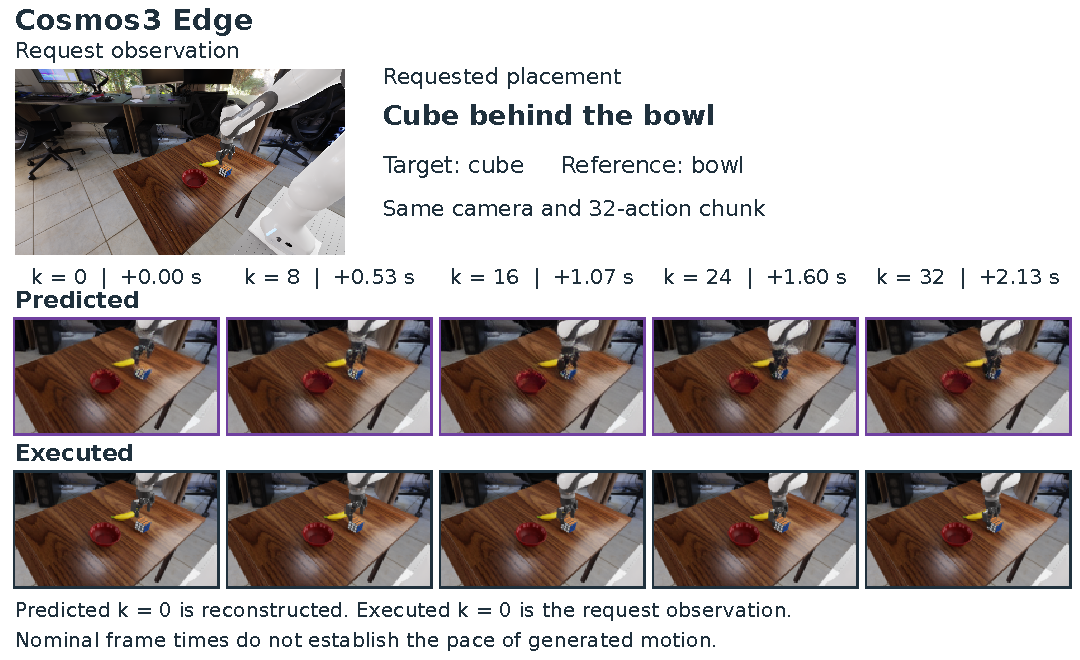
\includegraphics[width=\linewidth]{rev_forecast_edge_paper.pdf}
\caption{Cosmos3 Edge's prediction and policy rollout for its second action chunk in the cube-behind-bowl task. The contextual view locates the common crop used in both rows. Columns pair generated frame $k$ with the policy rollout after $k$ actions. Times follow the nominal 15\,Hz mapping. The first predicted frame is reconstructed. This example verifies the request, camera, and frame indexing, not the accuracy of predicted motion.}
\label{fig:forecast-example-edge}
\end{figure}

\begin{figure}[!ht]
\centering
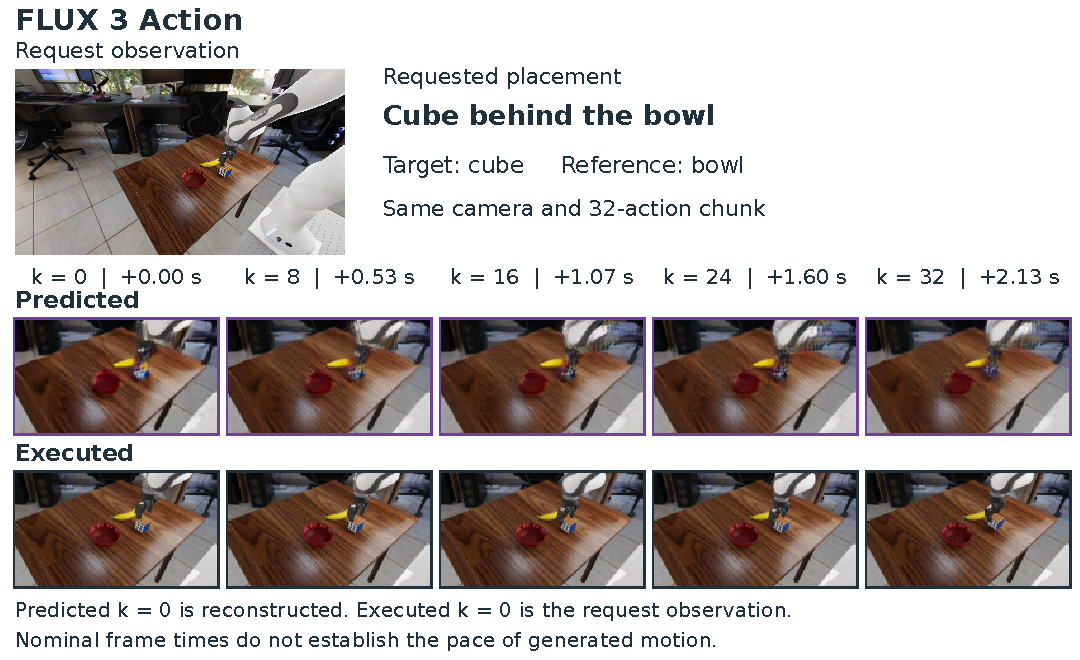
\includegraphics[width=\linewidth]{rev_forecast_flux_paper.pdf}
\caption{FLUX 3 Action on the same task and episode starting state as Figure~\ref{fig:forecast-example-edge}. Each model has already executed its own first chunk before the request shown here. The prediction becomes blurred while the policy rollout remains visually distinct. The layout and nominal frame correspondence follow the Edge example. FLUX jointly decodes its frames, including the reconstructed frame 0.}
\label{fig:forecast-example-flux}
\end{figure}

\begin{table}[!ht]
\centering
\small
\begin{tabular}{llll}
\toprule
Example & Readout & Final relation & Reference object \\
\midrule
Edge & Qwen & None & None \\
     & GLM & On top of & None \\
     & Adjudicated & None & None \\
\midrule
FLUX & Qwen & On top of & None \\
     & GLM & On top of & Cube (itself) \\
     & Adjudicated & On top of & None \\
\bottomrule
\end{tabular}
\caption{Original labels for the two illustrated forecasts. All six annotations identify object 3 (the cube) as moving upward, with no release. The table retains inconsistent or incomplete relation labels rather than repairing them after inspection. ``None'' is the saved label, not an independent determination that no relation holds.}
\label{tab:forecast-example-labels}
\end{table}

\FloatBarrier
\subsection{Ambiguity in the annotation materials}
\label{app:forecast-packets}

The original annotation materials reveal a separate measurement problem (Figure~\ref{fig:forecast-packets}). Direction arrows obscure some object numbers, and the cube's number overlaps the banana's circle in the right view. The original numbering is banana 1, bowl 2, and cube 3. Two of the six free-text responses misidentify these numbers: one Edge response exchanges the bowl and banana, and the FLUX adjudication calls the cube object 1. The structured moving-object field still identifies the cube in all six annotations, but one FLUX relation names the cube itself as its reference. Agreement on object selection therefore does not establish reliable interpretation of the spatial relation.

The contact sheets below summarize the stored forecasts for human inspection. They are not the exact input sequence shown to the VLMs, which received the numbered legend and eight generated frames at indices 0, 5, 9, 14, 18, 23, 27, and 32. No policy rollout images were supplied. The common packet layout also stretches Edge's decoded exterior views vertically. We preserve the original materials and labels so these presentation choices remain visible.

These observations do not show that the annotation layout caused the low agreement across the full study. They identify a plausible confound that should be removed before attributing an unreliable annotation to the model's predictions. Diagnostic evaluation depends on three separate steps: associating a prediction with the correct actions, presenting its contents unambiguously, and checking the accuracy of the extracted labels. The two verified examples address the first step and expose weaknesses in the second. Independent annotation checks are still needed for the third.

\begin{figure}[!ht]
\centering
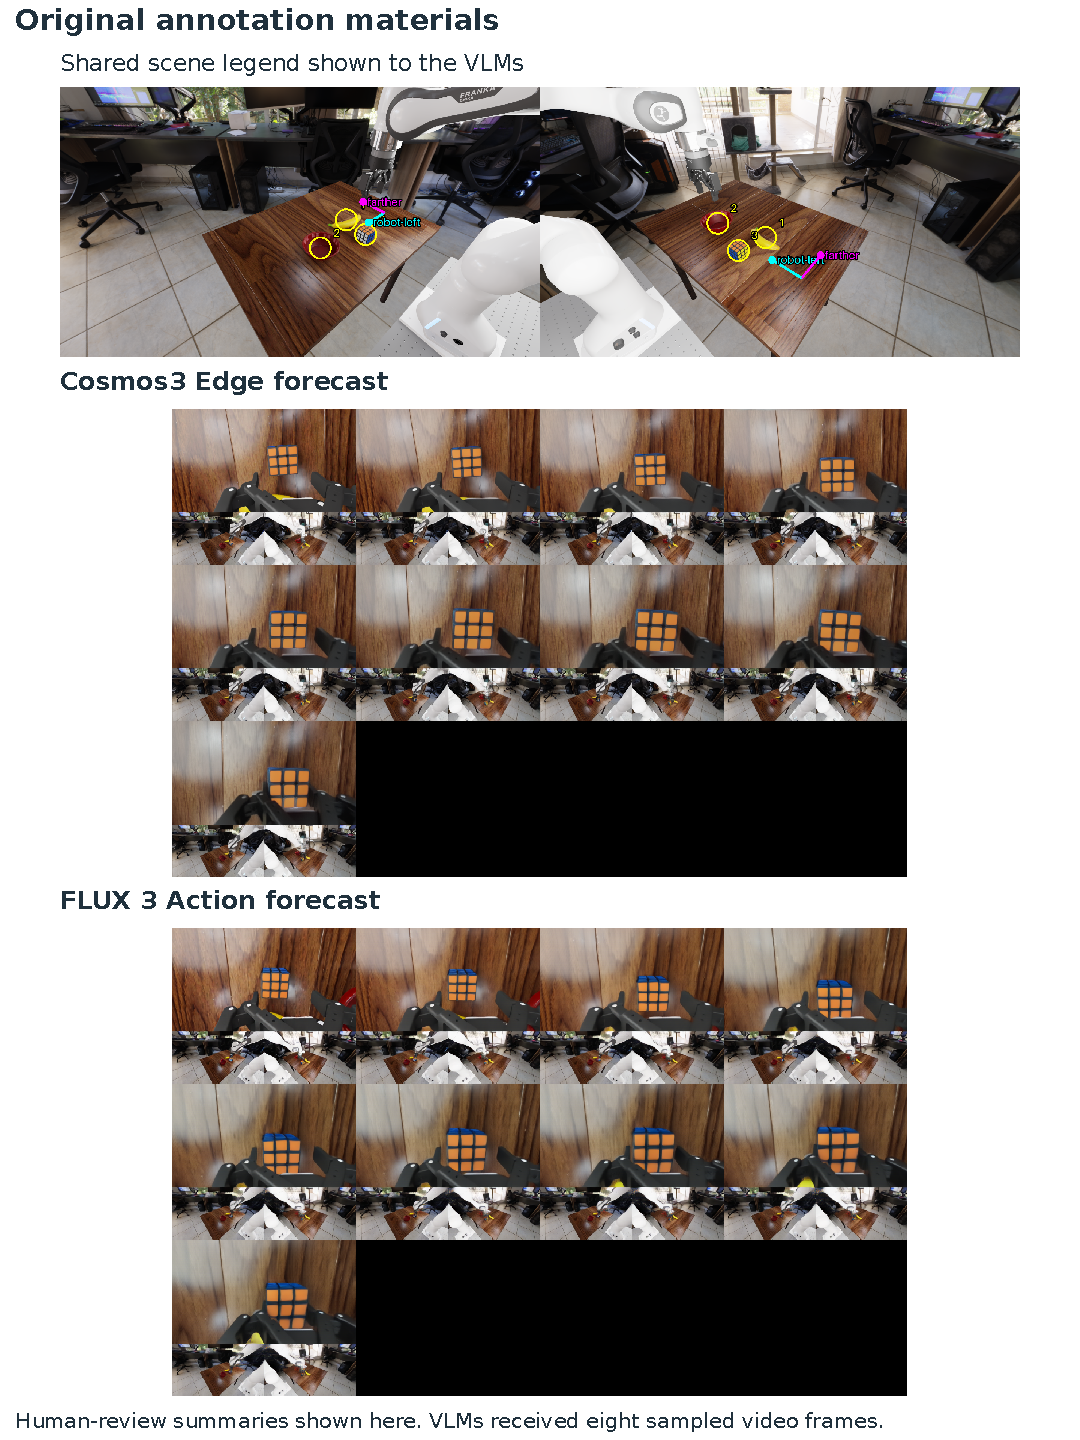
\includegraphics[width=.88\linewidth]{rev_forecast_packets_paper.pdf}
\caption{Original annotation imagery, preserved without correcting its labels. Both examples use the same episode-start legend. Some numbers overlap arrows or other objects' circles. The lower panels show the original human-review contact sheets for Edge and FLUX, with a wrist view above the two exterior views in each frame. These sheets sample every fourth generated frame, whereas the VLMs received the eight frames listed in the text. None of these images depicts a policy rollout.}
\label{fig:forecast-packets}
\end{figure}

\clearpage
\section{Matched instruction-understanding diagnostic}
\label{app:vqa}

\paragraph{Scope and protocol history.}
We conducted an inference-only diagnostic using the language components of the three evaluated policies. The diagnostic separates interpreting an instruction from judging a visible arrangement and generating actions. Version 1 (V1) tested scene relations (A), instruction interpretation (B), and whether an image matched an instruction (C). C was the prespecified primary diagnostic. Its near-constant negative answers made it inconclusive. We retain that result. After inspecting V1, we specified a bounded follow-up (V2) that enforced answer syntax, separated images from camera descriptions, and revised C's question. V2 is a diagnostic repair, not an independent replication or a replacement confirmatory primary test. Its specification and queries were frozen before evaluation. V1 remains unchanged.

V2 covers ten goals in the cube, butter, and mustard scenes: 30 exact DIR/TF/RF instructions and 24 physical starts. Bowl stacking is excluded because of the support/nesting ambiguity. We reuse 24 initial view sets and 48 fixed saved-rollout view sets, each with three synchronized camera views. No training, new robot episodes, or new scenes were added. All 6,552 evaluation queries completed without missing, truncated, or invalid-format answers.

Figure~\ref{fig:vqa-protocol} uses the three initial camera images from start \texttt{S4-C04}, verified byte-for-byte against the evaluated inputs. The full question, camera descriptions, image hashes, and example answers are archived with the paper revision.

\paragraph{Components and checkpoint lineage.}
The executed Nano reasoner matches Qwen3-VL-8B-Instruct. The executed Edge reasoner matches the released Edge base reasoner. Hashes of the loaded parameters, input processing, rendered prompts, and six development outputs established parity; identical pairs were evaluated once. FLUX's frozen shared encoder has the same weight files as Qwen3-VL-4B-Instruct. FLUX uses this component for text; standalone image QA is auxiliary and does not reproduce its policy's visual pathway. A separate Cosmos3-Nano base reasoner tested in V1 differs from the executed reasoner and is not treated as a matched pre-adaptation parent. These identities do not support degradation of the tested component weights during robot adaptation. Matched training data were unavailable, so this audit does not isolate training-recipe or co-training effects on the full policies.

\paragraph{Instruction interpretation and scoring.}
B2 returns the requested target object, reference object, and target-relative relation. Schema-constrained decoding fixes the JSON structure and available vocabulary without pruning to the correct answer. This is an assisted test: format validity is guaranteed, while exact tuple accuracy requires all three fields to be correct. We use the existing language heads, BF16 inference, greedy decoding, and at most 256 new tokens. There is no trained probe.

The four input conditions are text alone (T), text with camera-orientation descriptions (H), text with initial images (I), and both images and descriptions (IH). Each image contrast holds the surrounding text fixed. B2's correct answer is defined by the instruction, not by the arrangement visible in the image. Its scoring therefore does not require visual-answerability labels, even when images are present.

Text-only answers are generated once per unique instruction and reported as finite counts. They are not independent observations for each physical start. Image accuracy averages starts within goals, goals within scenes, and scenes equally. Intervals use 10,000 physical-start bootstrap samples within scene (seed 6106). They condition on the three fixed scenes and wording templates. Image-versus-text contrasts reuse the same text-only answer and paired bootstrap samples; their uncertainty does not include variation over new language templates.

\begin{table}[htbp]
\centering\small
\caption{B2 exact tuple scores. Text-only columns count correct answers out of ten instructions per form. IH columns show equal-scene accuracy with images and camera descriptions. A dagger marks FLUX image results as auxiliary.}
\label{tab:vqa-full}
\begin{tabular}{@{}lrrr@{\qquad}rrr@{}}
\toprule
& \multicolumn{3}{c}{Text only: correct / 10}
& \multicolumn{3}{c}{Images + descriptions: \%}\\
Component & DIR & TF & RF & DIR & TF & RF\\
\midrule
Nano & 10 & 10 & 10 & 100.0 & 100.0 & 89.9\\
Edge & 6 & 8 & 4 & 30.6 & 48.3 & 23.3\\
FLUX & 10 & 10 & 4 & $100.0^\dagger$ & $100.0^\dagger$ & $41.7^\dagger$\\
\bottomrule
\end{tabular}
\end{table}

\paragraph{Interpretation errors and controls.}
Table~\ref{tab:vqa-full} shows RF disadvantages for Edge and FLUX from text alone. All six FLUX RF errors are converse relations. Edge also errs on DIR and TF. V1 rejected 375 of 414 Edge B responses for format, whereas V2 enforces syntax. The protocols differ in decoding, so their score difference is not a model improvement.

Nano is correct on all 30 instructions in T and H. IH produces eight converse errors: five butter-right and three cube-behind starts. RF accuracy decreases by 10.1 percentage points relative to H (95\% interval 5.2--14.6). I produces four butter-right converse errors and one butter-on-top support-label swap. Its RF decrease relative to T is 6.9 points (1.4--12.5). Camera descriptions alone change no Nano answers. Their additional effect with images is unresolved (IH minus I: $-3.1$ points, interval $-8.0$ to $+1.7$). These effects are concentrated in specific instructions.

\begin{table}[htbp]
\centering\small
\caption{Additional B2 controls. H and I entries follow DIR/TF/RF order. H gives counts out of ten; I gives equal-scene accuracy. Placement controls move the reference clause without changing converse vocabulary. FLUX image entries are auxiliary.}
\label{tab:vqa-controls}
\begin{tabular}{@{}lcccc@{}}
\toprule
& H: correct / 10 & I: accuracy (\%) & \multicolumn{2}{c}{Placement controls}\\
Component & DIR / TF / RF & DIR / TF / RF & T: correct / 16 & IH: \%\\
\midrule
Nano & 10 / 10 / 10 & 100.0 / 100.0 / 93.1 & 16 & 100.0\\
Edge & 5 / 10 / 4 & 38.9 / 46.2 / 23.3 & 13 & 50.5\\
FLUX & 10 / 10 / 3 & $97.2 / 100.0 / 41.7^\dagger$ & 16 & $100.0^\dagger$\\
\bottomrule
\end{tabular}
\end{table}

Nano and FLUX answer every placement-control item correctly. Edge scores 5/8 reference-early and 8/8 reference-late instructions in T. Its IH reference-early deficit is 17.7 points (10.4--25.0). These controls use a different sentence construction from RF and do not rule out general noun-order effects.

\paragraph{Inconclusive current-state judgments and visual review.}
C2 asks whether the current image shows the requested arrangement. It counterbalances the codes for match and nonmatch and permits an insufficient-evidence response. Answers remain nearly constant nonmatch under both code orders. Balanced accuracy is 48.5--50.1\% across tested components and image banks; always answering nonmatch yields 50\%. At most one of eleven matched truth-changing frame pairs is classified correctly on both frames. These outcomes cannot establish wording robustness or general spatial incompetence. The bounded pass stops without further prompt repair.

Unlike B2, A and C depend on whether the relation is visible. No human reviewed their images. Blinded machine review covered 36 of 72 view sets, or 120 of 240 frame--goal items. Only twelve sets received two reviewers. Some agents failed to return forms; one primary reviewer used programmatic pixel analysis after image-display failure. A further form that used the evaluated Nano backbone was excluded from the primary mask. All 39 reviewed initial items were judged answerable, but only 27 of 81 secondary items were answerable to every reviewer. These partial machine judgments remain provisional. Reviewed-mask rescoring leaves C2 near chance, but does not substitute for human validation. The QA results characterize component behavior; they neither observe the policies' internal goal representation nor establish that a QA error causes an action failure.

\end{document}
